\documentclass{beamer}
%%%%%%%%%%%%%%%%%%%%%%%%%%%%%%%%%%%%%%%%%%%%%%%%%%%%%%%%%%%%%%%%%%%%%%%%%%%%%%%%%%%%%%%%%%%%%%%%%%
\setbeamertemplate{navigation symbols}{}
\usepackage{beamerthemeshadow}
\usefonttheme{serif}
%%%%%%%%%%%%%%%%%%%%%%%%%%%%%%%%%%%%%%%%%%%%%%%%%%%%%%%%%%%%%%%%%%%%%%%%%%%%%%%%%%%%%%%%%%%%%%%%%%
\usepackage{graphicx}
\graphicspath{ {res/} }
%%%%%%%%%%%%%%%%%%%%%%%%%%%%%%%%%%%%%%%%%%%%%%%%%%%%%%%%%%%%%%%%%%%%%%%%%%%%%%%%%%%%%%%%%%%%%%%%%%
\usepackage{polyglossia}
\setdefaultlanguage{armenian}
\setotherlanguages{english}
\usepackage{fontspec}
\newfontfamily\armenianfont{DejaVu Sans}
%%%%%%%%%%%%%%%%%%%%%%%%%%%%%%%%%%%%%%%%%%%%%%%%%%%%%%%%%%%%%%%%%%%%%%%%%%%%%%%%%%%%%%%%%%%%%%%%%%
\usepackage{minted}
\setminted[cpp]{fontsize=\footnotesize}
\setmonofont{Consolas}
%%%%%%%%%%%%%%%%%%%%%%%%%%%%%%%%%%%%%%%%%%%%%%%%%%%%%%%%%%%%%%%%%%%%%%%%%%%%%%%%%%%%%%%%%%%%%%%%%%
\usepackage{xltxtra}
\usepackage{hyperref}
%%%%%%%%%%%%%%%%%%%%%%%%%%%%%%%%%%%%%%%%%%%%%%%%%%%%%%%%%%%%%%%%%%%%%%%%%%%%%%%%%%%%%%%%%%%%%%%%%%
\usetheme{Luebeck}
\usecolortheme{crane}
%%%%%%%%%%%%%%%%%%%%%%%%%%%%%%%%%%%%%%%%%%%%%%%%%%%%%%%%%%%%%%%%%%%%%%%%%%%%%%%%%%%%%%%%%%%%%%%%%%
\definecolor{HTDark}{rgb}{0.04706, 0.13725, 0.26667} % primary color
\definecolor{HTLight}{rgb}{0.3686, 0.5255, 0.6235}   % secondary color
\setbeamercolor{palette primary}{bg=HTDark,fg=white}
\setbeamercolor{palette secondary}{bg=HTDark,fg=white}
\setbeamercolor{palette tertiary}{bg=HTDark,fg=white}
\setbeamercolor{palette quaternary}{bg=HTDark,fg=white}
\setbeamercolor{structure}{fg=HTDark} % itemize, enumerate, etc
\setbeamercolor{section in toc}{fg=HTDark} % TOC sections
\setbeamercolor{block title}{fg=white,bg=HTDark}
\setbeamercolor{block body}{fg=white, bg=HTLight}
\setbeamercolor{subsection in head/foot}{bg=HTLight,fg=white}
%%%%%%%%%%%%%%%%%%%%%%%%%%%%%%%%%%%%%%%%%%%%%%%%%%%%%%%%%%%%%%%%%%%%%%%%%%%%%%%%%%%%%%%%%%%%%%%%%%


\begin{document}

\title[AbstractFactory]{Նախագծման Ձևանմուշներ։ AbstractFactory}
\author[Հրաչյա Թանդիլյան\copyright]{Հրաչյա Թանդիլյան}
\date{2020}

%-------------------------------------------------------------------------------------------------
\begin{frame}
\titlepage
\end{frame}
%-------------------------------------------------------------------------------------------------

\section{Նպատակը}
%-------------------------------------------------------------------------------------------------
\begin{frame}\frametitle{AbstractFactory}
\begin{block}{Նպատակը}
    Տրամադրում է ինտերֆեյս միմյանց հետ կապված կամ միմյանցից կախված օբյեկտների
    ընտանիքներ ստեղծելու համար, առանց նշելու նրանց կոնկրետ տիպը:
\end{block}
\vfill
Նաև հայտնի է որպես
\begin{itemize}
    \item Kit
\end{itemize}
\end{frame}
%-------------------------------------------------------------------------------------------------

\subsection{Մոտիվացիան}
%-------------------------------------------------------------------------------------------------
\begin{frame}\frametitle{Մոտիվացիան}
\begin{center}
    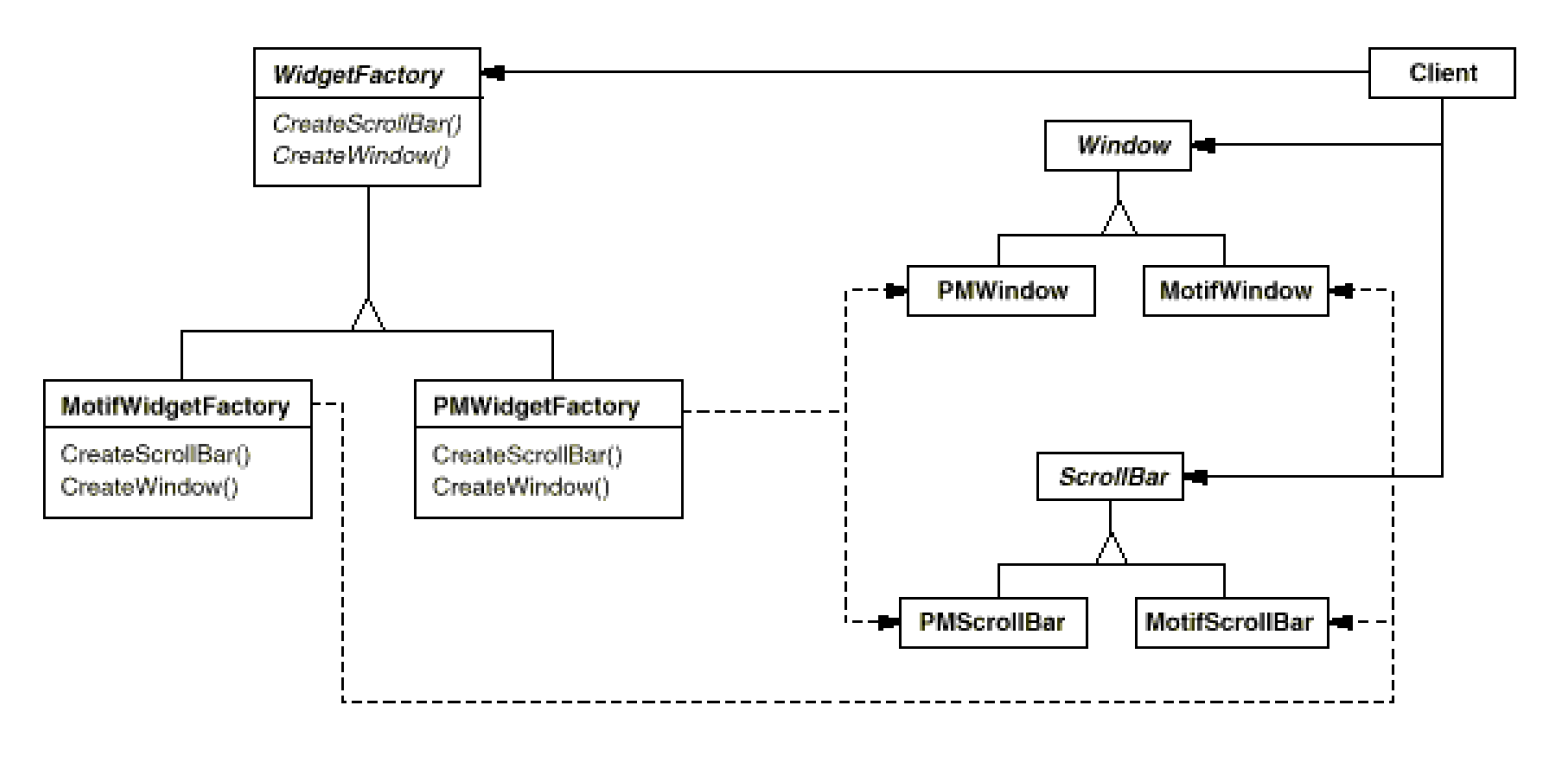
\includegraphics[scale=0.4]{motivation.png}
\end{center}
\end{frame}
%-------------------------------------------------------------------------------------------------

\subsection{Կիրառելիությունը}
%-------------------------------------------------------------------------------------------------
\begin{frame}\frametitle{Կիրառելիությունը}
Այս Ն.Ձ. պետք է օգտագործել երբ.
\vfill
\begin{enumerate}
    \item Համակարգը պետք է անկախ լինի իր կոմպոնենտների ստեղծումից և ներկայացումից: \pause \vfill
    \item Համակարգը պետք է աշխատի կոմպոնենտների բազմաթիվ ընտանիքներից միայն մեկի հետ: \pause \vfill
    \item Անհրաժեշտ է ստիպել, որ միևնույն ընտանիքի կոմպոնենտներին համապատասխան
    օբյեկտները աշխատեն միայն միմյանց հետ: \pause \vfill
    \item Անհրաժեշտ է տրամադրել կոմպոնենտների դասերի գրադարան, այնպես որ բացահայտվի
    միայն նրանց ինտերֆեյսը և ոչ թե իրականացումը:
\end{enumerate}
\end{frame}
%-------------------------------------------------------------------------------------------------

\section{Կառուցվածքը}
%-------------------------------------------------------------------------------------------------
\begin{frame}\frametitle{Կառուցվածքը}
\begin{center}
    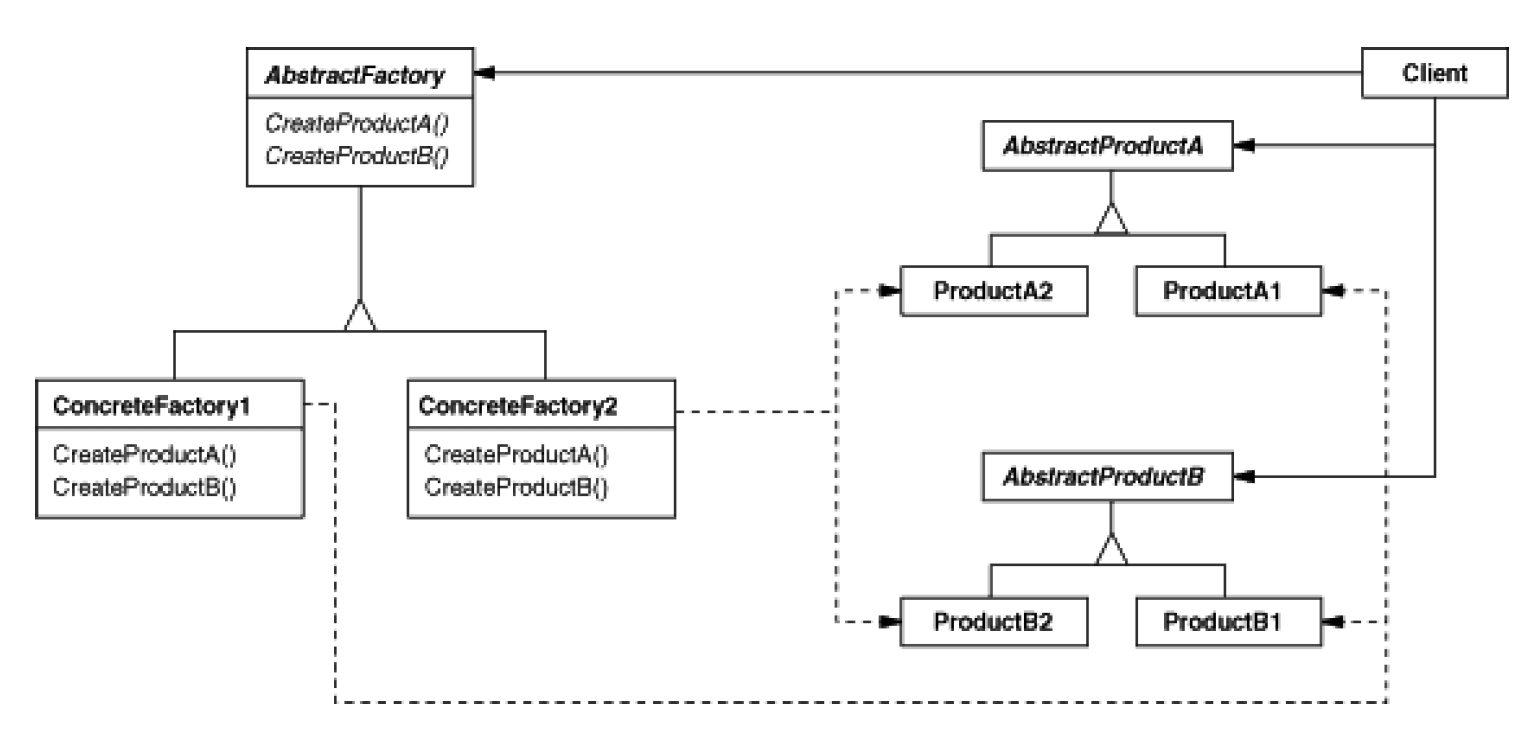
\includegraphics[scale=0.4]{structure.png}
\end{center}
\end{frame}
%-------------------------------------------------------------------------------------------------

\subsection{Հետևանքները}
%-------------------------------------------------------------------------------------------------
\begin{frame}\frametitle{Հետևանքները}
Այս Ն.Ձ. ունի հետևյալ առավելություններն ու թերությունները.
\vfill
\begin{enumerate}
    \item Առանձնացնում է կոնկրետ դասերը: \pause \vfill
    \item Հեշտացնում է կոմպոնենտների ընտանիքների փոխարինումը: \pause \vfill
    \item Ապահովում է կայունություն կոմպոնենտների միջև: \pause \vfill
    \item Դժվարեցնում է նոր տիպի կոմպոնենտների ավելացումը:
\end{enumerate}
\end{frame}
%-------------------------------------------------------------------------------------------------

\section{Իրականացումը}
%-------------------------------------------------------------------------------------------------
\begin{frame}\frametitle{Իրականացումը}
\begin{enumerate}
    \item Factory–ները որպես Singleton: \pause \vfill
    \item Կոմպոնենտների ստեղծումը: \pause \vfill
    \item Ընդլայնելի Factory-ների ստեղծումը:
\end{enumerate}
\end{frame}
%-------------------------------------------------------------------------------------------------

\subsection{Օրինակ}
%-------------------------------------------------------------------------------------------------
\begin{frame}[fragile]\frametitle{Օրինակ}
\begin{english}
\begin{minted}{cpp}
class MazeFactory {

public:
    MazeFactory();

    virtual Maze* MakeMaze() const { return new Maze; }

    virtual Wall* MakeWall() const { return new Wall; }

    virtual Room* MakeRoom(int n) const { return new Room(n); }

    virtual Door* MakeDoor(Room* r1, Room* r2) const {
        return new Door(r1, r2);
    }
};
\end{minted}
\end{english}
\end{frame}
%-------------------------------------------------------------------------------------------------

%-------------------------------------------------------------------------------------------------
\begin{frame}[fragile]\frametitle{Օրինակ}
\begin{english}
\begin{minted}[fontsize=\scriptsize]{cpp}
Maze* MazeGame::CreateMaze(MazeFactory& factory) {
    Maze* aMaze = factory.MakeMaze();

    Room* r1 = factory.MakeRoom(1);
    Room* r2 = factory.MakeRoom(2);
    aMaze->AddRoom(r1); aMaze->AddRoom(r2);

    Door* aDoor = factory.MakeDoor(r1, r2);
    r1->SetSide(East, aDoor); r2->SetSide(West, aDoor);

    r1->SetSide(North, factory.MakeWall());
    r1->SetSide(South, factory.MakeWall());
    r1->SetSide(West, factory.MakeWall());
    r2->SetSide(North, factory.MakeWall());
    r2->SetSide(East, factory.MakeWall());
    r2->SetSide(South, factory.MakeWall());

    return aMaze;
}
\end{minted}
\end{english}
\end{frame}
%-------------------------------------------------------------------------------------------------

%-------------------------------------------------------------------------------------------------
\begin{frame}[fragile]\frametitle{Օրինակ}
\begin{english}
\begin{minted}{cpp}
class EnchantedMazeFactory : public MazeFactory {

public:
    EnchantedMazeFactory();

    virtual Room* MakeRoom(int n) const {
        return new EnchantedRoom(n, CastSpell());
    }

    virtual Door* MakeDoor(Room* r1, Room* r2) const {
        return new DoorNeedingSpell(r1, r2);
    }

protected:
    Spell* CastSpell() const;
};
\end{minted}
\end{english}
\end{frame}
%-------------------------------------------------------------------------------------------------

%-------------------------------------------------------------------------------------------------
\begin{frame}[fragile]\frametitle{Օրինակ}
\begin{english}
\begin{minted}{cpp}
class BombedMazeFactory : public MazeFactory {

public:
    BombedMazeFactory();

    virtual Room* MakeRoom(int n) const {
        return new RoomWithABomb(n);
    }

    Wall* MakeWall () const {
        return new BombedWall;
    }
};

MazeGame game;
BombedMazeFactory factory;
game.CreateMaze(factory);
\end{minted}
\end{english}
\end{frame}
%-------------------------------------------------------------------------------------------------

\section{Առնչվող Ձևանմուշները}
%-------------------------------------------------------------------------------------------------
\begin{frame}\frametitle{Առնչվող Նախագծման Ձևանմուշները}
\begin{itemize}
    \item Factory Method \vfill
    \item Prototype \vfill
    \item Singleton
\end{itemize}
\end{frame}
%-------------------------------------------------------------------------------------------------

\end{document}
